La implementación de las fuentes de tensión de \SI{12}{\volt} y \SI{-12}{\volt} se realizó en base a los circuitos integrados \texttt{LM2576} y \texttt{LM2577}. Se propuso la construcción de dos circuitos independinetes, con el fin de no consumir toda la corriente de una sola fuente.

\subsection{Fuente reductora de tensión}
El diseño propuesto en la figura \ref{fig.fte_12} corresponde a la configuración reductora de tensión cuya entrada es \SI{+30}{\volt}, y su salida \SI{+12}{\volt}. Debido a la dificultad de conseguir el modelo \textit{LM2565-12}, se decidió utilizar la versión ajustable, la cuál implica anexar dos resistencias de realimentación $R_2$ y $R_3$ según el esquema. El inductor $L_2$ y el capacitor $C_3$ permiten reducir el riple de la tensión de salida.


\begin{figure}
	\centering
	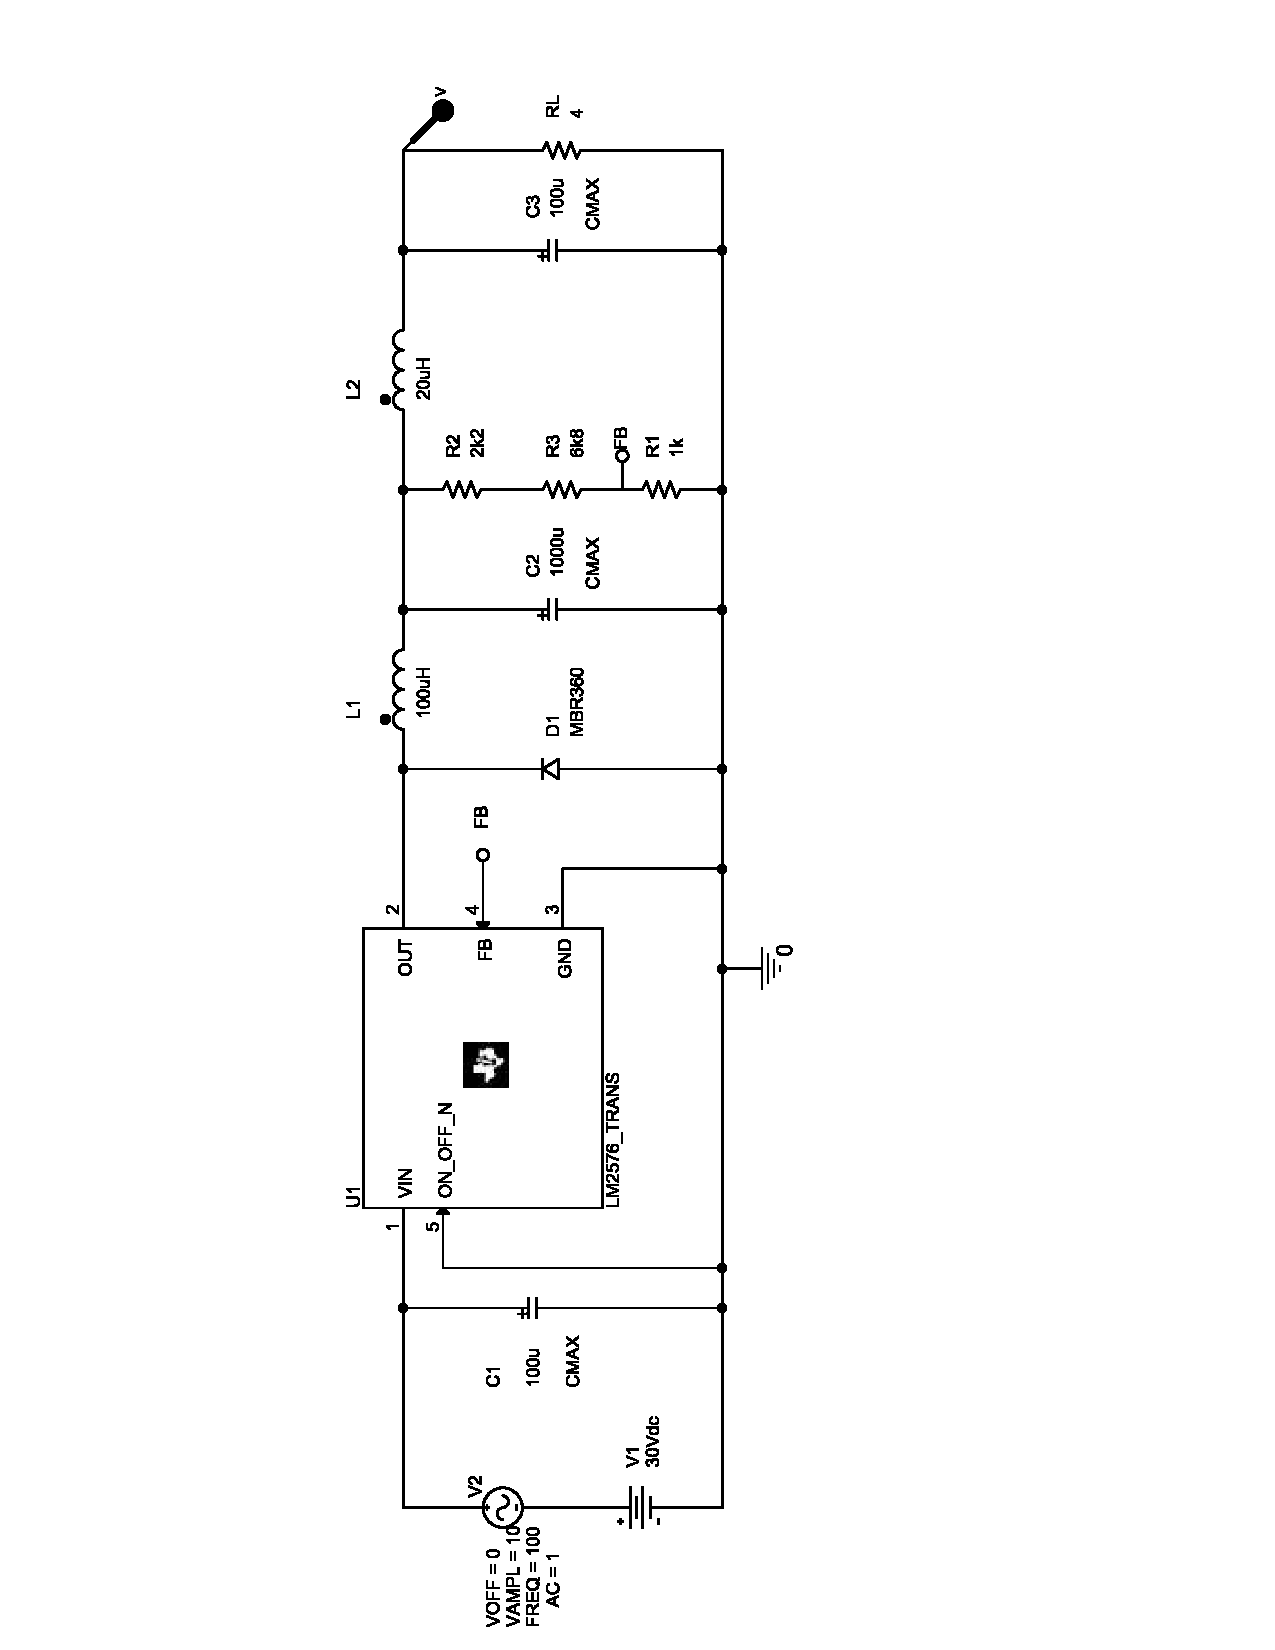
\includegraphics[scale=0.5]{fte_12_esquema.pdf}
	\caption{Fuente reductora de tensión.}
	\label{fig.fte_12}
\end{figure}


Debido a que la fuente de entrada puede variar en un 20\%, en la simulación se anexó una fuente alterna en serie para analizar el comportamiento de la salida ante alteraciones de $V_E$. La salida resultante se muetra en la figura \ref{fig.fte_salida_12}, observándose una variación del orden de decenas de $\SI{}{\milli\volt}$.

\HgraficarPNG{0.5}{fte_12_salida}{Salida de la fuente reductora de tensión}{fig.fte_salida_12}


\subsection{Fuente elevadora de tensión}

Para el circuito elevador, desde -30V a -12V, se propuso el diseño de la figura . 
No se logró realizar la simulación debido a la inexistencia del modelo de   \texttt{LM2577} en PSpice. 
La elección de los componentes se detalla en la nota de aplicación , aunque sus valores podrán variar empíricamente.

\HgraficarPNG{0.5}{lm2577}{Fuente elevadora de tensión.}{fig.fte_elevadora}

